\chapter{Lecture 16 - Curve Fitting and Interpolation with Built-in MATLAB Tools}
\label{ch:lec16n}
\section{Objectives}
The objectives of this lecture are to:
\begin{itemize}
\item Demonstrate the use of MATLAB built-in tools for polynomial curve fitting.
\item Demonstrate the use of MATLAB built-in interpolation functions.
\end{itemize}
\setcounter{lstannotation}{0}

\section{Polynomial Curve Fitting in MATLAB}

MATLAB has an easy-to-use tool for polynomial curve fitting: \lstinline[style=myMatlab]{p = polyfit(x,y,m)}.  In this function, $x$ and $y$ are vectors describing the data to be fit and $m$ is the order of the polynomial fit desired.  The function returns a vector $p$ which is a vector of length $(m+1)$ and stores the coefficients for the polynomial fit:
\begin{equation*}
f(x) = p(1)x^{m} + p(2)x^{m-1} + \cdots + p(m+1)x^0
\end{equation*}  
This might seem awkward and/or unexpected, but do not despair, MATLAB provides a convenient function to evaluate this polynomial: \lstinline[style=myMatlab]{polyval(p,x)}.  

\vspace{0.25cm}

\noindent\textbf{Example:} The percent of households that own at least one computer in selected years from 1981 to 2010, according to the U.S. Census Bureau, is listed in Table \ref{tab:lec16n-ex1}.

\begin{table}
\begin{tabular}{|l|l|l|l|l|l|l|l|l|l|l|}
\hline
Year & 1981 & 1984 & 1989 & 1993 & 1997 & 2000 & 2001 & 2003 & 2004 & 2010 \\ \hline
\% w/computers & 0.5 & 8.2 & 15 & 22.9 & 36.6 & 51 & 56.3 & 61.8 & 65 & 76.7 \\ \hline
\end{tabular}
\caption[][-1.25cm]{Percentage of U.S. households that own at least one computer.}
\label{tab:lec16n-ex1}
\end{table} 

\vspace{0.15cm}

\noindent Use MATLAB built-in functions to create a 3\textsuperscript{rd}-order polynomial interpolant and estimate the percent ownership of computers in 2008 and 2013. 
\begin{lstlisting}[style=myMatlab,name=lec16n-ex1]
clear
clc
close 'all'

base_year = 1981;
year = [1981,1984, 1989, 1993, 1997,...
    2000, 2001, 2003, 2004, 2010];

pct_w_comp = [0.5, 8.2, 15, 22.9, 36.6, 51,...
    56.3, 61.8, 65, 76.7];

year = year-base_year; /*!\annotation{lst:ann16n-1}!*/
m = 3;
p = polyfit(year,pct_w_comp,m);

x1 = 2008 - base_year; 
x2 = 2013 - base_year;

fprintf('Estimated percent ownership in %d is %g percent.\n',...
    x1+base_year, polyval(p,x1));
fprintf('Estimated percent ownership in %d is %g percent.\n',...
    x2+base_year, polyval(p,x2));

\end{lstlisting}
\marginnote{

\vspace{-4.20cm}

\noindent \ref{lst:ann16n-1} Translating the variable \lstinline[style=myMatlab]{years} in this way provides a better conditioned system of equations.  Readers are encouraged to eliminate this translation and observe the result.

}
The resulting polynomial fit is shown in Figure \ref{fig:lec16n-ex1}.  The estimated percent computer ownership in 2008 is 74.25\% and in 2013 is 80.00\%.
\begin{marginfigure}
\includegraphics{lec16n-ex1.png}
\caption{A 3\textsuperscript{rd}-order polynomial fit using \lstinline[style=myMatlab]{polyval()} and \lstinline[style=myMatlab]{polyfit()}.}
\label{fig:lec16n-ex1}
\end{marginfigure}

\section{Interpolation with MATLAB}
Although we have thoroughly covered curve fitting and extended that application to interpolation, we really have not yet discussed any methods that can be reliably used for data interpolation.  Readers may find this somewhat confusing since they almost certainly have carried out simple linear interpolation at some point in their lives.  There are, of course, more sophisticated and reliable algorithms for data interpolation but we will not cover them in detail in this text.  Instead, we will rely on built-in MATLAB tools that are readily available.  The workhorse function for one-dimensional interpolation is: \lstinline[style=myMatlab]{interp1(x,y,x_q,method)}.  The first two inputs comprise the data to be interpolated.  The third input variable, \lstinline[style=myMatlab]{x_q}, is a vector of \emph{query points} where interpolated data is desired.  

MATLAB provides several methods including:
\begin{enumerate}
\item \lstinline[style=myMatlab]{'linear'}: This method requires at least 2 points in the data vectors and produces a piece-wise-linear interpolant.

\item \lstinline[style=myMatlab]{'nearest'}:  As the name implies this method will interpolate elements of the query vector to the nearest neighbor in the data vector.  This results in a piece-wise-constant interpolation.

\item \lstinline[style=myMatlab]{'next'} or \lstinline[style=myMatlab]{'previous'}:  Produces a piece-wise-constant interpolation, as the name implies, to the data point after or before the query point along the $x$ axis.

\item A handful of higher-order and spline interpolants:
\begin{enumerate}
\item \lstinline[style=myMatlab]{'cubic'} 
\item \lstinline[style=myMatlab]{'pchip'} and 
\item \lstinline[style=myMatlab]{'spline'} 
\end{enumerate}
to list a few.  

\end{enumerate}
Readers seeking more details should, of course, consult the MATLAB documentation.  An example usage is shown below.

\vspace{0.25cm}

\noindent\textbf{Example: } The following data shows the power of a diesel engine at different engine speeds.

\begin{table}
\begin{tabular}{|l|l|l|l|l|l|l|l|l|l|l|}
\hline
Engine RPM & 1200 & 1500 & 2000 & 2500 & 3000 & 3250 & 3500 & 3750 & 4000 & 4400 \\\hline
Engine Power (hp) & 65 & 130 & 185 & 225 & 255 & 266 & 275 & 272 & 260 & 230 \\ \hline
\end{tabular}
\end{table}
Use MATLAB to create an interpolation of the data.  Plot the estimated engine power from 1200 to 4400 RPM.  Estimate the engine power at 2300 RPM.

The MATLAB code needed to do this is presented in the listing below.

\begin{lstlisting}[style=myMatlab,name=ex3]
clear
clc
close 'all'

x = [1200, 1500, 2000, 2500, 3000,...
    3250, 3500, 3750,4000, 4400];
y = [65, 130, 185, 225, 255, 266,...
    275, 272, 260, 230];

method = 'pchip';

f_int = @(xi) interp1(x,y,xi,method);

xMin = min(x); xMax = max(x); Nx = 1000;
X_space = linspace(xMin, xMax, Nx);

figure(4)
plot(x,y,'ro',...
    X_space,f_int(X_space),'-b',...
    'linewidth',3)
title('MATLAB Interpolation','fontsize',16,...
    'fontweight','bold');
xlabel('Engine Speed [RPM]','fontsize',14,'fontweight','bold');
ylabel('Power [hp]','fontsize',14,'fontweight','bold');
grid on;
set(gca,'fontsize',12,'fontweight','bold');
axis([xMin xMax 0.5*min(y) 1.25*max(y)]);

x1 = 2300;
fprintf('Estimated hp at %d rpm: %g \n',...
    x1, f_int(x1));
\end{lstlisting}
A plot of the interpolation is shown in Figure \ref{fig:lec16n-ex3}.  The estimated engine power at 2300 RPM is 210.43 horsepower using this interpolation method.  Readers are encouraged to experiment with alternative interpolation methods to see how each performs.
\begin{marginfigure}
\includegraphics{lec16n-ex3.png}
\caption{Interpolated curve of engine power versus engine speed.}
\label{fig:lec16n-ex3}
\end{marginfigure}
\subsection{Interpolation in 2D and 3D}
It is often necessary to carry out interpolation on surfaces and in volumes.  Perhaps the most important application is in data visualization.  A numeric simulation based on the finite difference or finite element method can be used, for example, to find the temperature on a surface or a volume.  The temperature, being a function, is usually represented as a vector. In many formulations the temperature vector corresponds to the temperature at discrete points within the surface or volume.  What we \emph{want} as engineers is the ability to see a smooth representation of the temperature throughout the domain; perhaps we also carry out some kind of calculation based on the integral or derivatives of that temperature field.  The way much of this is done, is via interpolation.  We create an interpolant to represent the function throughout the domain and it is the interpolant that is subjected to the differentiation or integration processes.  Data \emph{post processing} of this sort is an essential activity that allows us to gain insight from our numerical solutions.    
\begin{marginfigure}
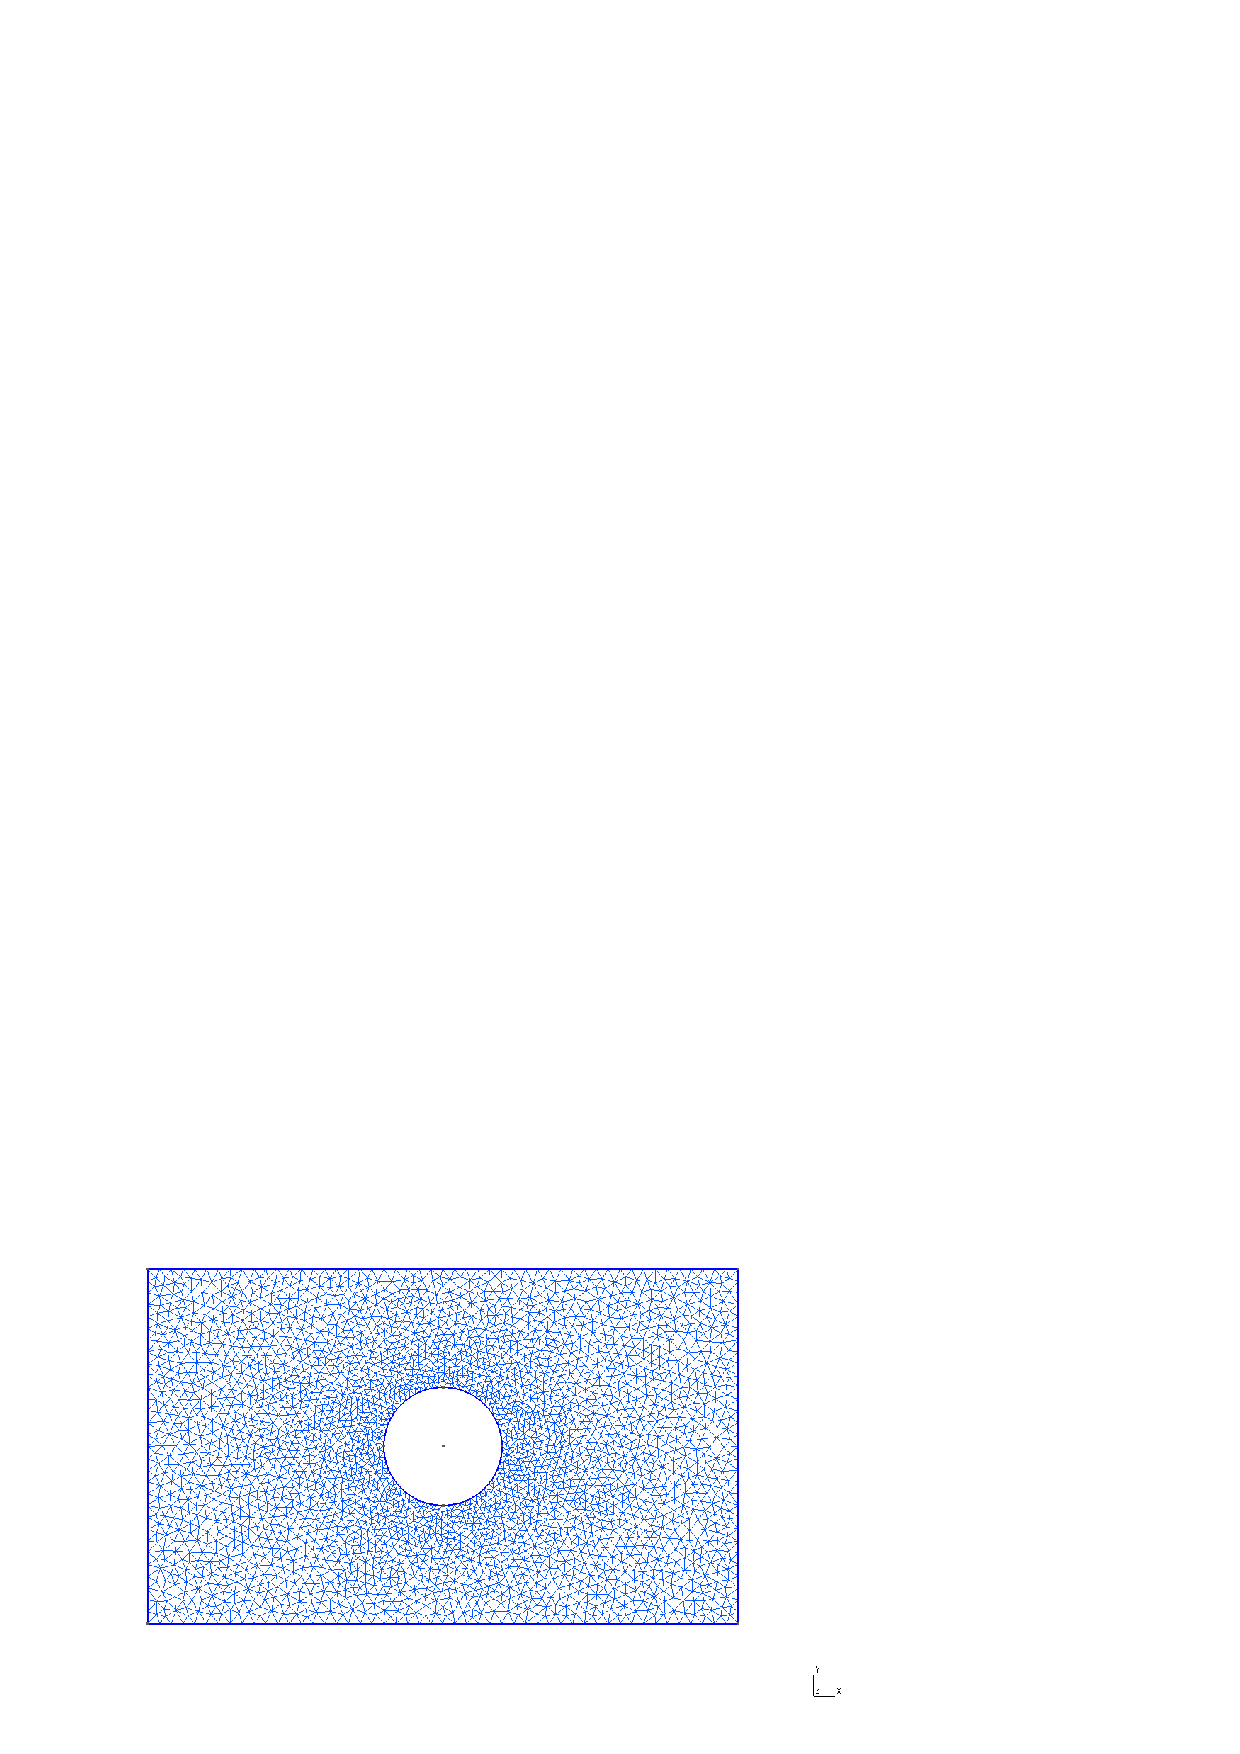
\includegraphics{discretization.png}
\caption{A discretized domain for a finite element method.}
\label{fig:lec16n-discretization}
\end{marginfigure}
Consider a rectangular domain discretized as part of the finite element method shown in Figure \ref{fig:lec16n-discretization}.  When the analysis is completed, we want to represent the temperature throughout the domain as a smooth function.  As is shown in the MATLAB listing below, we can use the built-in function---\lstinline[style=myMatlab]{scatteredInterpolant()}---to create the smooth interpolated representation shown in Figure \ref{fig:lec16n-ex4-temp}.
\begin{marginfigure}
\includegraphics{lec16n-ex4-temp.png}
\caption{Interpolated temperature data.}
\label{fig:lec16n-ex4-temp}
\end{marginfigure}

\begin{lstlisting}[style=myMatlab,name=lec16n-ex4]
clear
clc
close 'all'
% load data from FEM analysis
load('fem_data.mat');
% create an interpolant over the 2D domain
TempField = scatteredInterpolant(gcoord(:,1),gcoord(:,2),T);
xMin = min(gcoord(:,1)); xMax = max(gcoord(:,1));
yMin = min(gcoord(:,2)); yMax = max(gcoord(:,2));
% make a smooth plot of temperature over the domain
Nx = 200; Ny = 200;
X = linspace(xMin,xMax,Nx); Y = linspace(yMin,yMax,Ny);
[XX,YY] = meshgrid(X,Y);
figure(1)
surf(XX,YY,TempField(XX,YY),'edgecolor','none');
title('Temperature Field','fontsize',16,...
    'fontweight','bold')
xlabel('X','fontsize',14,'fontweight','bold');
ylabel('Y','FontSize',14, 'FontWeight','bold');
zlabel('T ^{\circ}C','FontSize',14,'FontWeight','bold');
\end{lstlisting}
